\documentclass[a4paper, 12pt, fleqn]{article}
\usepackage[utf8]{inputenc}
\usepackage[english]{babel}
\usepackage[margin=1in, bmargin=1in]{geometry}
\usepackage{amsmath, amssymb, amsfonts, graphicx, commath}

\title{\textsc{Power usage CNN on the Khavas Vim 3}}
\author{Anton Pham, Levi van der Griendt}
\date{\today}
%%%%%%%%%%%%%%%%%%%%%%%%%%%%%%%%%%%%%%%%%%%%%%%%%%%%%%%%%%%%%%%%%%%%%%%%%%%%%%%%%%%%%%%%%%%%%%%%%%%%%%%%

\begin{document} \maketitle


\section{Introduction}
Embedded systems are commonly used in power-constrained environments, and the efficient management of power consumption is crucial for their performance and longevity. In particular, governors are Operating System (OS) sub-routines that are responsible for the power management of embedded systems. As a result, significant and careful research is needed to discover the most optimized power consumption model for embedded system. Consequentially, detailed reports about the power-performance reciprocity of specific architectures on governors are needed to provide more understanding into the power management capabilities of the governors.

In this report, we present a power-performance characterization of Convolutional Neural Networks architectures (CNNs) on the Khadas VIM 3 board, which is an embedded platform based on the Amlogic A311D Heterogeneous Multi-Processor System on Chip (HMPSoC). We evaluate the governor using five image classification CNNs: AlexNet, GoogleNet, MobileNet, ResNet50, and SqueezeNet. These CNNs are executed using the ARM-CL framework on the ARM-based HMPSoC in the Khadas VIM 3 board. Our goal is to provide insights into how different power-efficiency knobs in the board affect the power and performance of CNNs.


The HMPSoC in the Khadas VIM 3 board has a hexa-core asymmetric ARM big.Little multi-core CPU with two CPU clusters, big and Little, and a dual-core Mali G52 MP4 GPU. The maximum frequency for the big CPU cluster, Little CPU cluster, and GPU is 1.8 GHz, 2.2 GHz, and 0.8 GHz, respectively. A 4 GB LPDDR4 main memory supports the HMPSoC. The platform runs Android v9.0 with kernel v4.9, and we run ARM-CL v21.02 on top of it.

In this work, we use a modified research version of ARM-CL called Pipe-All, which allows for simultaneous inference on both CPU and GPU cores using a software pipeline. The parameterized code for Pipe-All allows the user to redistribute the workload between the big CPU cluster, the Little CPU cluster, and the GPU. The governor we design uses this workload distribution feature from Pipe-All as a power management knob. Additionally, we use Dynamic Voltage and Frequency Scaling (DVFS) as another power management knob. DVFS technology changes a core's voltage and frequency at run-time, allowing governors to tailor the performance of a core to match the requirements and save power.



\section{Method}
In this power-performance characterization report, we evaluated the power and performance of five state-of-the-art image classification Convolutional Neural Networks (CNNs) on the Khadas VIM 3 board. The CNNs used in this study were AlexNet, GoogleNet, MobileNet, ResNet50, and SqueezeNet. These CNNs were executed using the ARM-CL framework on an ARM-based Heterogeneous Multi-Processor Systems on Chip (HMPSoC) known as the Amlogic A311D HMPSoC, which is integrated in the Khadas Vim 3 embedded platform.

The HMPSoC used in this study contains a hexa-core asymmetric ARM big-little multicore CPU with two CPU clusters, Big and Little. The quad-core big CPU cluster contains four high-power, high-performance A73 cores, while the dual-core Little CPU cluster contains two low-power, low-performance A53 cores. The HMPSoC also contains a dual-core Mali G52 MP4 GPU. The maximum frequency for the big CPU cluster, Little CPU cluster, and GPU is 1.8 GHz, 2.2 GHz, and 0.8 GHz, respectively. A 4 GB LPDDR4 main memory supports the HMPSoC. In software, the platform was running Android v9.0 with kernel v4.9. We ran ARM-CL v21.02 on top of it.

To perform the power-performance characterization, we used a modified research version of the ARM-CL library called Pipe-All (Aghapour, \& Torab, 2022). This version of the library allows for simultaneous inference on both CPU and GPU cores using a software pipeline. The parameterized code for Pipe-All allows the user to redistribute the workload between the big CPU cluster, the Little CPU cluster, and the GPU. The Governor used in this work used this workload distribution feature from Pipe-All as a power management knob. In addition to the workload distribution feature, we also used Dynamic Voltage and Frequency Scaling (DVFS) as a power management knob. DVFS technology changes a core’s voltage and frequency at run-time, allowing Governors to tailor the performance of a core to match the requirements and save power. The Governor used in this work also used DVFS as a power management knob.

To physically set up the board, we followed the instructions provided in the guide. This included using a laptop running Ubuntu 20.04 and a USB-A port to connect to the Khadas VIM3 board, as well as other required peripheral equipment. 

We collected power and performance data for each CNN using the governor and power management knobs described above, by recording the minimum, maximum, and median power consumption (W) and the average frame latency during the inference interval. The numbers of frames used for the Little CPU, Big CPU, and GPU are 80, 100, and 100 frames consecutively. Every CNN was run on the a combination of pipelines in which each cluster was configured as the first target in the pipeline. For the Little and Big CPUs, the maximum frequency level was also changed incrementally based on the permitted options of frequencies for each of the CPU clusters, to record the power-performance data to analyze the complete relationship between power consumption and performance level. Furthermore, These data were then used to create charts and graphs to visually represent the power and performance characteristics of the CNNs on the Khadas VIM 3 board.

In this report, we provided generalized insights on how the power and performance move with different power-efficiency knobs in the board. The results of this study can be used to inform the design of governors and power management strategies for embedded systems operating in power-constrained environments.    

Another test to be done is looking at how the ordering matters and how this impacts performance and energy consumption. For this test, we used a simple one-frequency test. We used 1704000 hz for the big A73 cores and 1200000 HZ for the smaller A53 cores. This is just for measuring the same thing. There is also we will partition things into even blocks by first testing each core alone then in duo in all possible configurations and last with all 3 in 9 different setups. We can get a good insight into how to partition. and how different time it takes from different parts of the CCN's we tested. 


\section{Results}
The results of the experiment were analyzed and presented through several plots. Figure 1 illustrates the relationship between the power consumption and latency of the CNNs. The graph shows that as performance increases, so does the power consumption, with a similar trend observed in Resnet50 and SqueezeNet.

On the other hand, Figure 2 shows the relationship between power consumption and latency, with fewer data intervals and lower values. This trend is consistent with the other graphs in this category. 

\begin{figure}[ht]
\centering
\begin{minipage}{.5\textwidth}
  \centering
  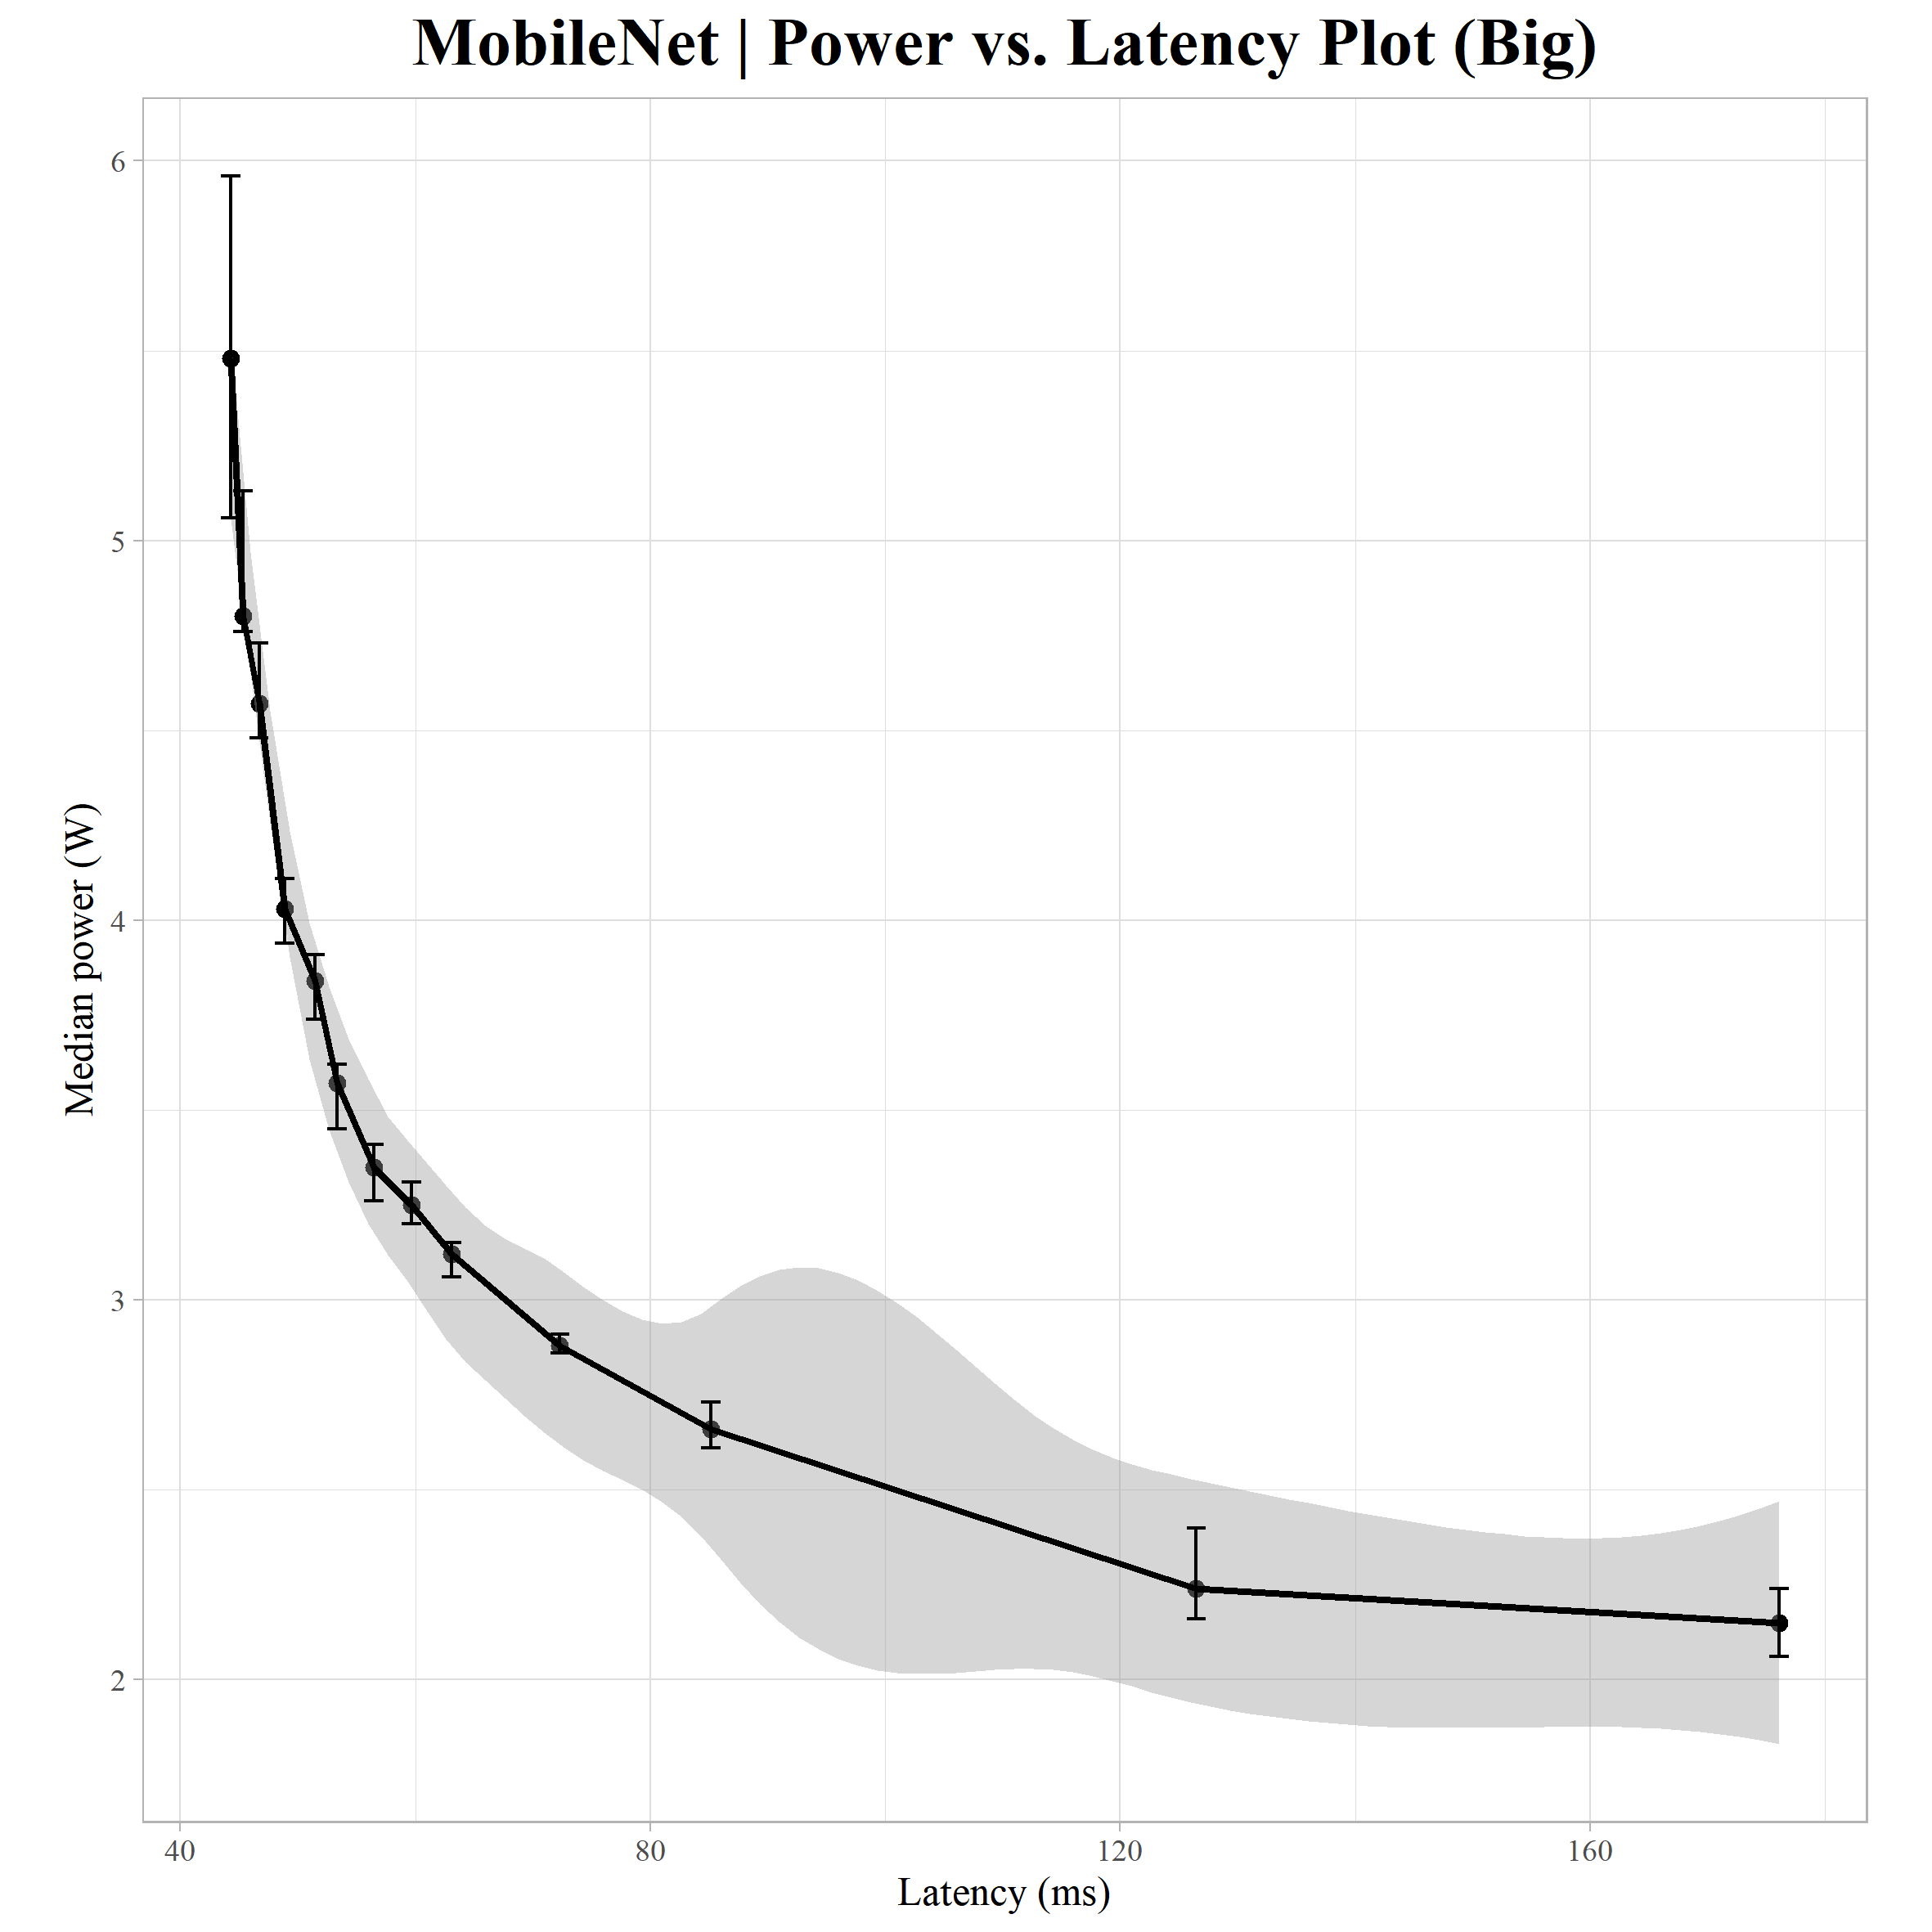
\includegraphics[width=1\linewidth]{Big/big - MobileNet.png}
  \caption{MobileNet on the Big core}
  \label{fig:big_1}
\end{minipage}%
\begin{minipage}{.5\textwidth}
  \centering
  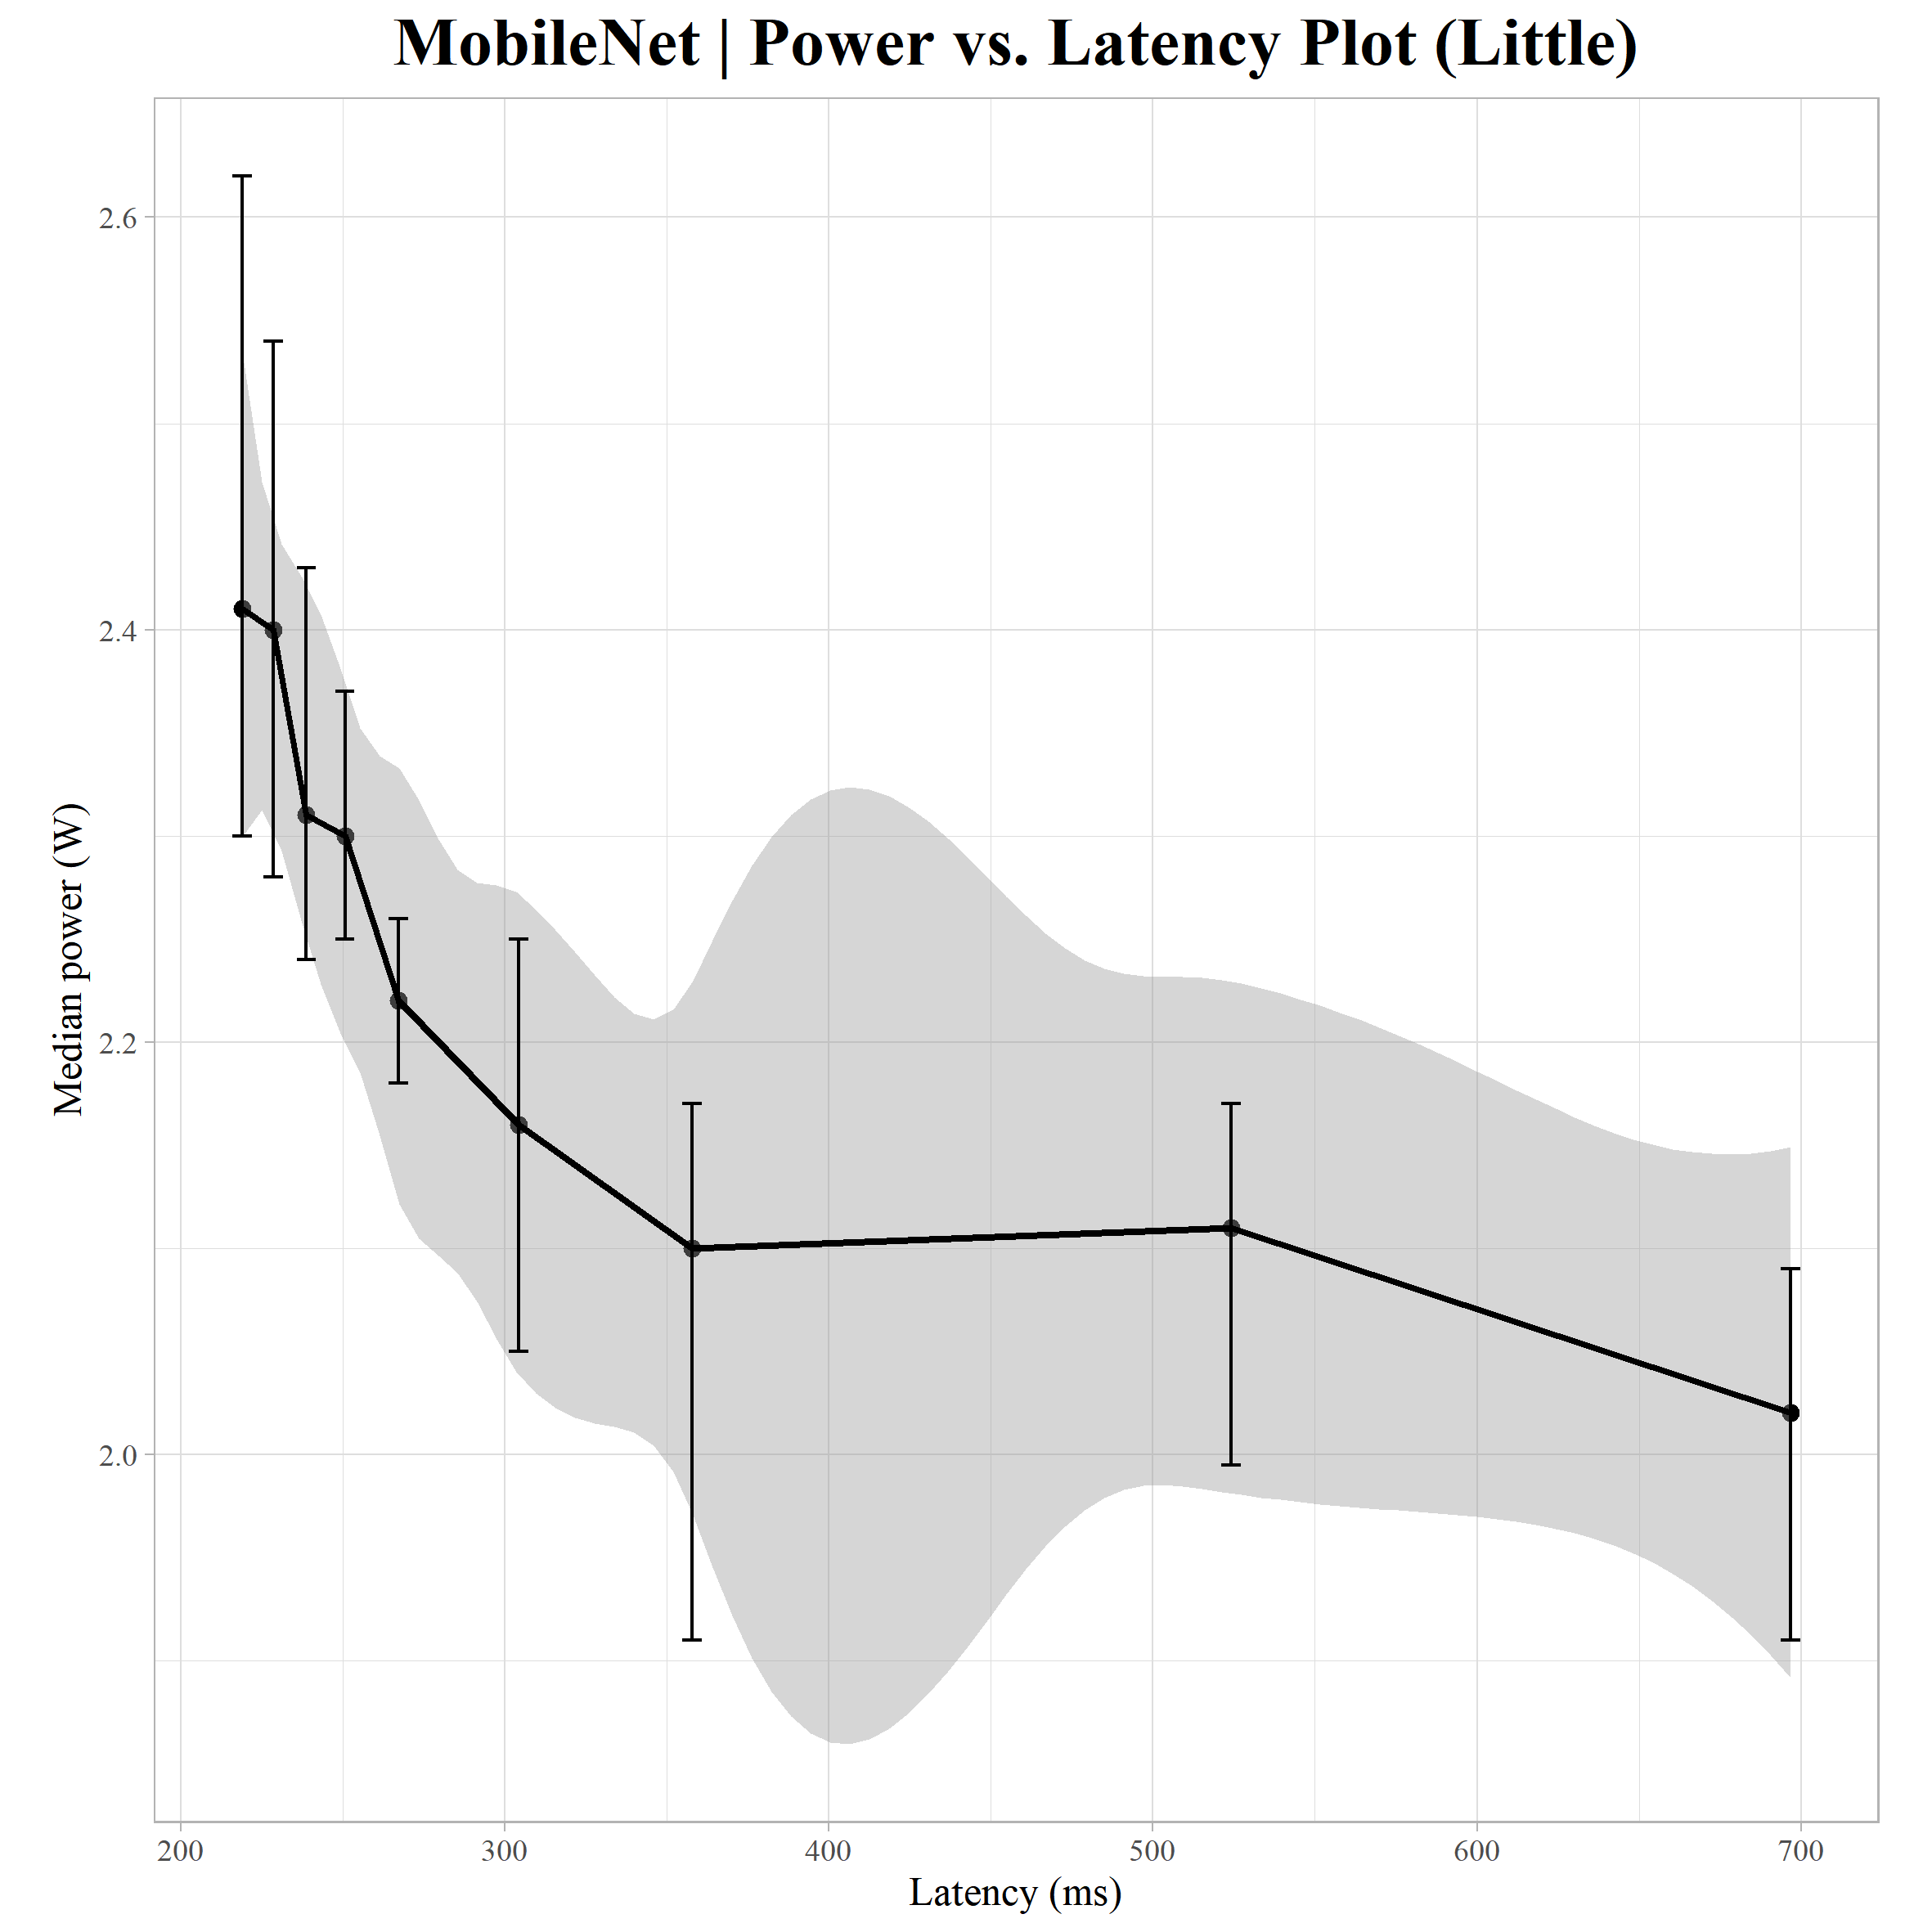
\includegraphics[width=1\linewidth]{Little/lit - MobileNet.png}
  \caption{MobileNet on the Little core}
  \label{fig:lit_1}
\end{minipage}
\end{figure}

Figure 3 and 4 demonstrate the effect of partitioning the CNN parts among the different cores on performance and latency. It is evident that there is a significant change in performance, with low performance resulting in lower latency. This suggests that it is more efficient to run on low performance on the Big CPU rather than high performance on the Little CPU for most CNNs, with the exception of AlexNet. Additionally, there is a fluctuation at the center of the slope in Figure 4, which is also observed in the GoogleNet graph on the same frequency.

\begin{figure}[ht]
\centering
\begin{minipage}{.5\textwidth}
  \centering
  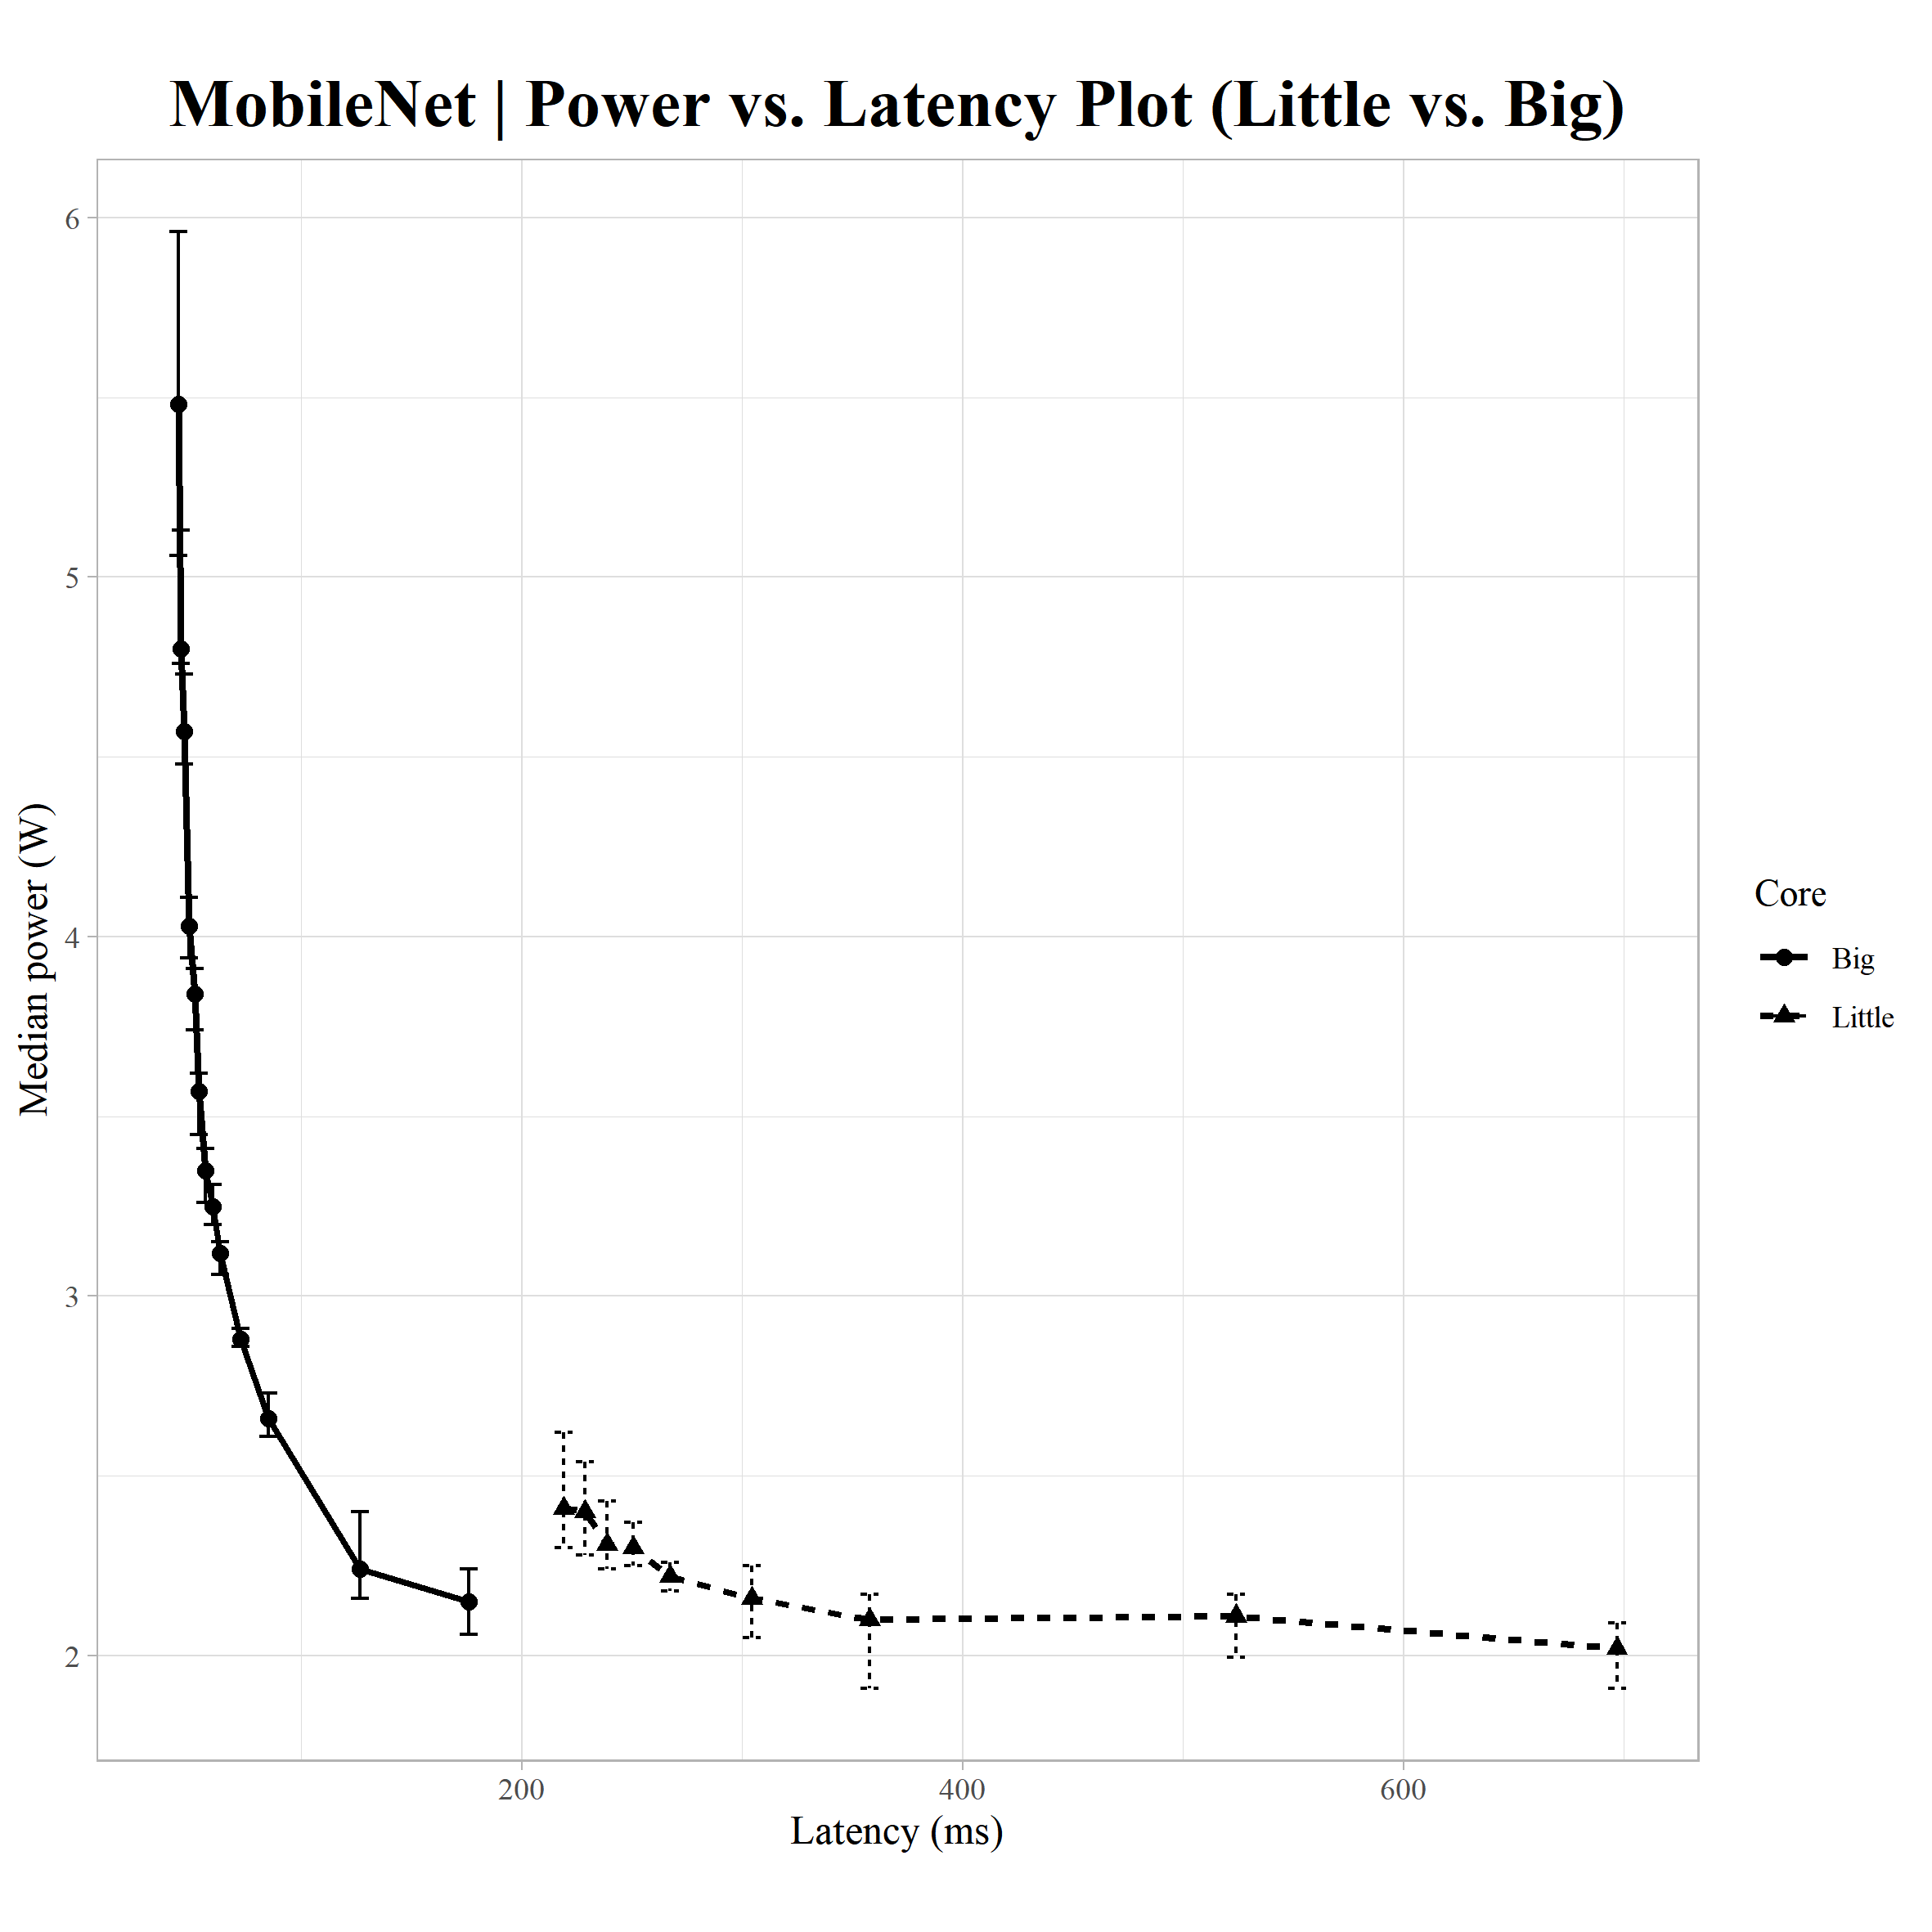
\includegraphics[width=1\linewidth]{LittleBig/litBig - MobileNet.png}
  \caption{MobileNet on both CPUs}
  \label{fig:litBig_1}
\end{minipage}%
\begin{minipage}{.5\textwidth}
  \centering
  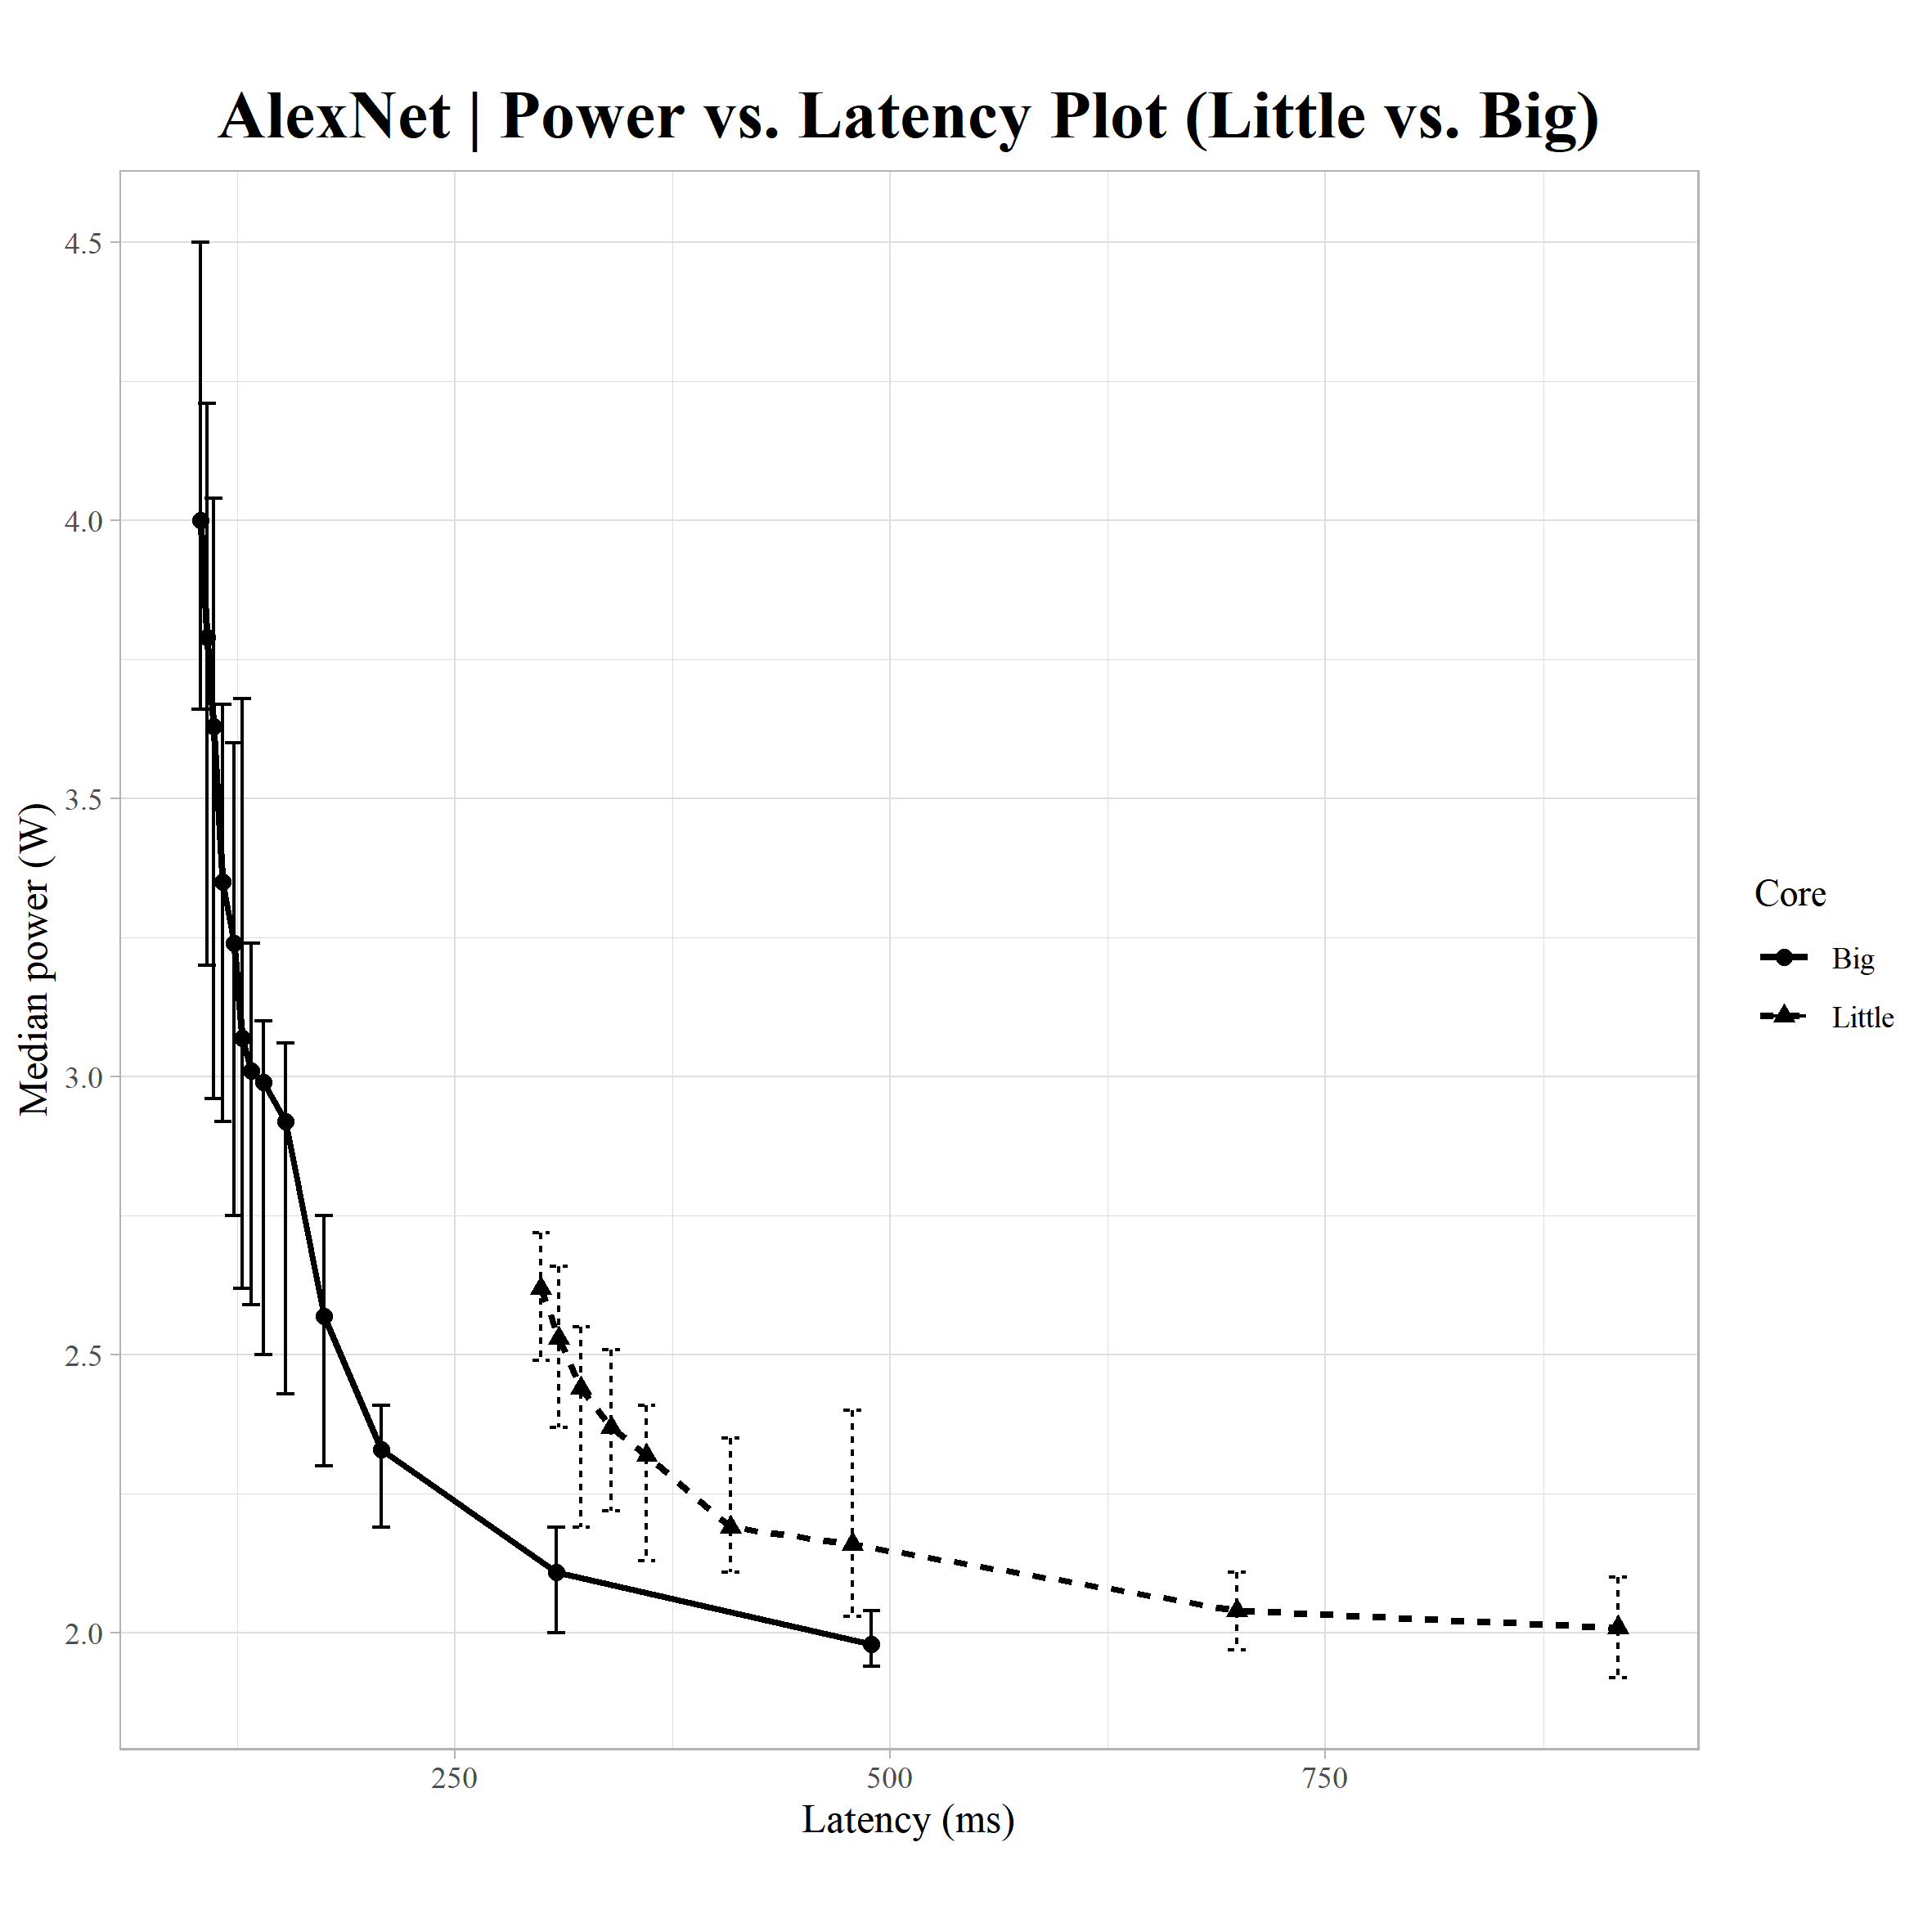
\includegraphics[width=1\linewidth]{LittleBig/litBig - AlexNet.png}
  \caption{AlexNet on both CPUs}
  \label{fig:litBig_2}
\end{minipage}
\end{figure}

Lastly, Figure 5 presents the GPU performance in terms of frames per second per watt, showing the efficiency of the GPU. Additionally, the graph highlights that the Big CPU is more power efficient when high speed is required. We decided to look at the performance efficiency of the maximum and minimum CPUs and GPU, by evaluating the ratio $\frac{FPS}{W}$, because $FPS = \frac{1}{Throughput}$ we could observe how efficient they are.

\begin{figure}[ht]
    \centering
    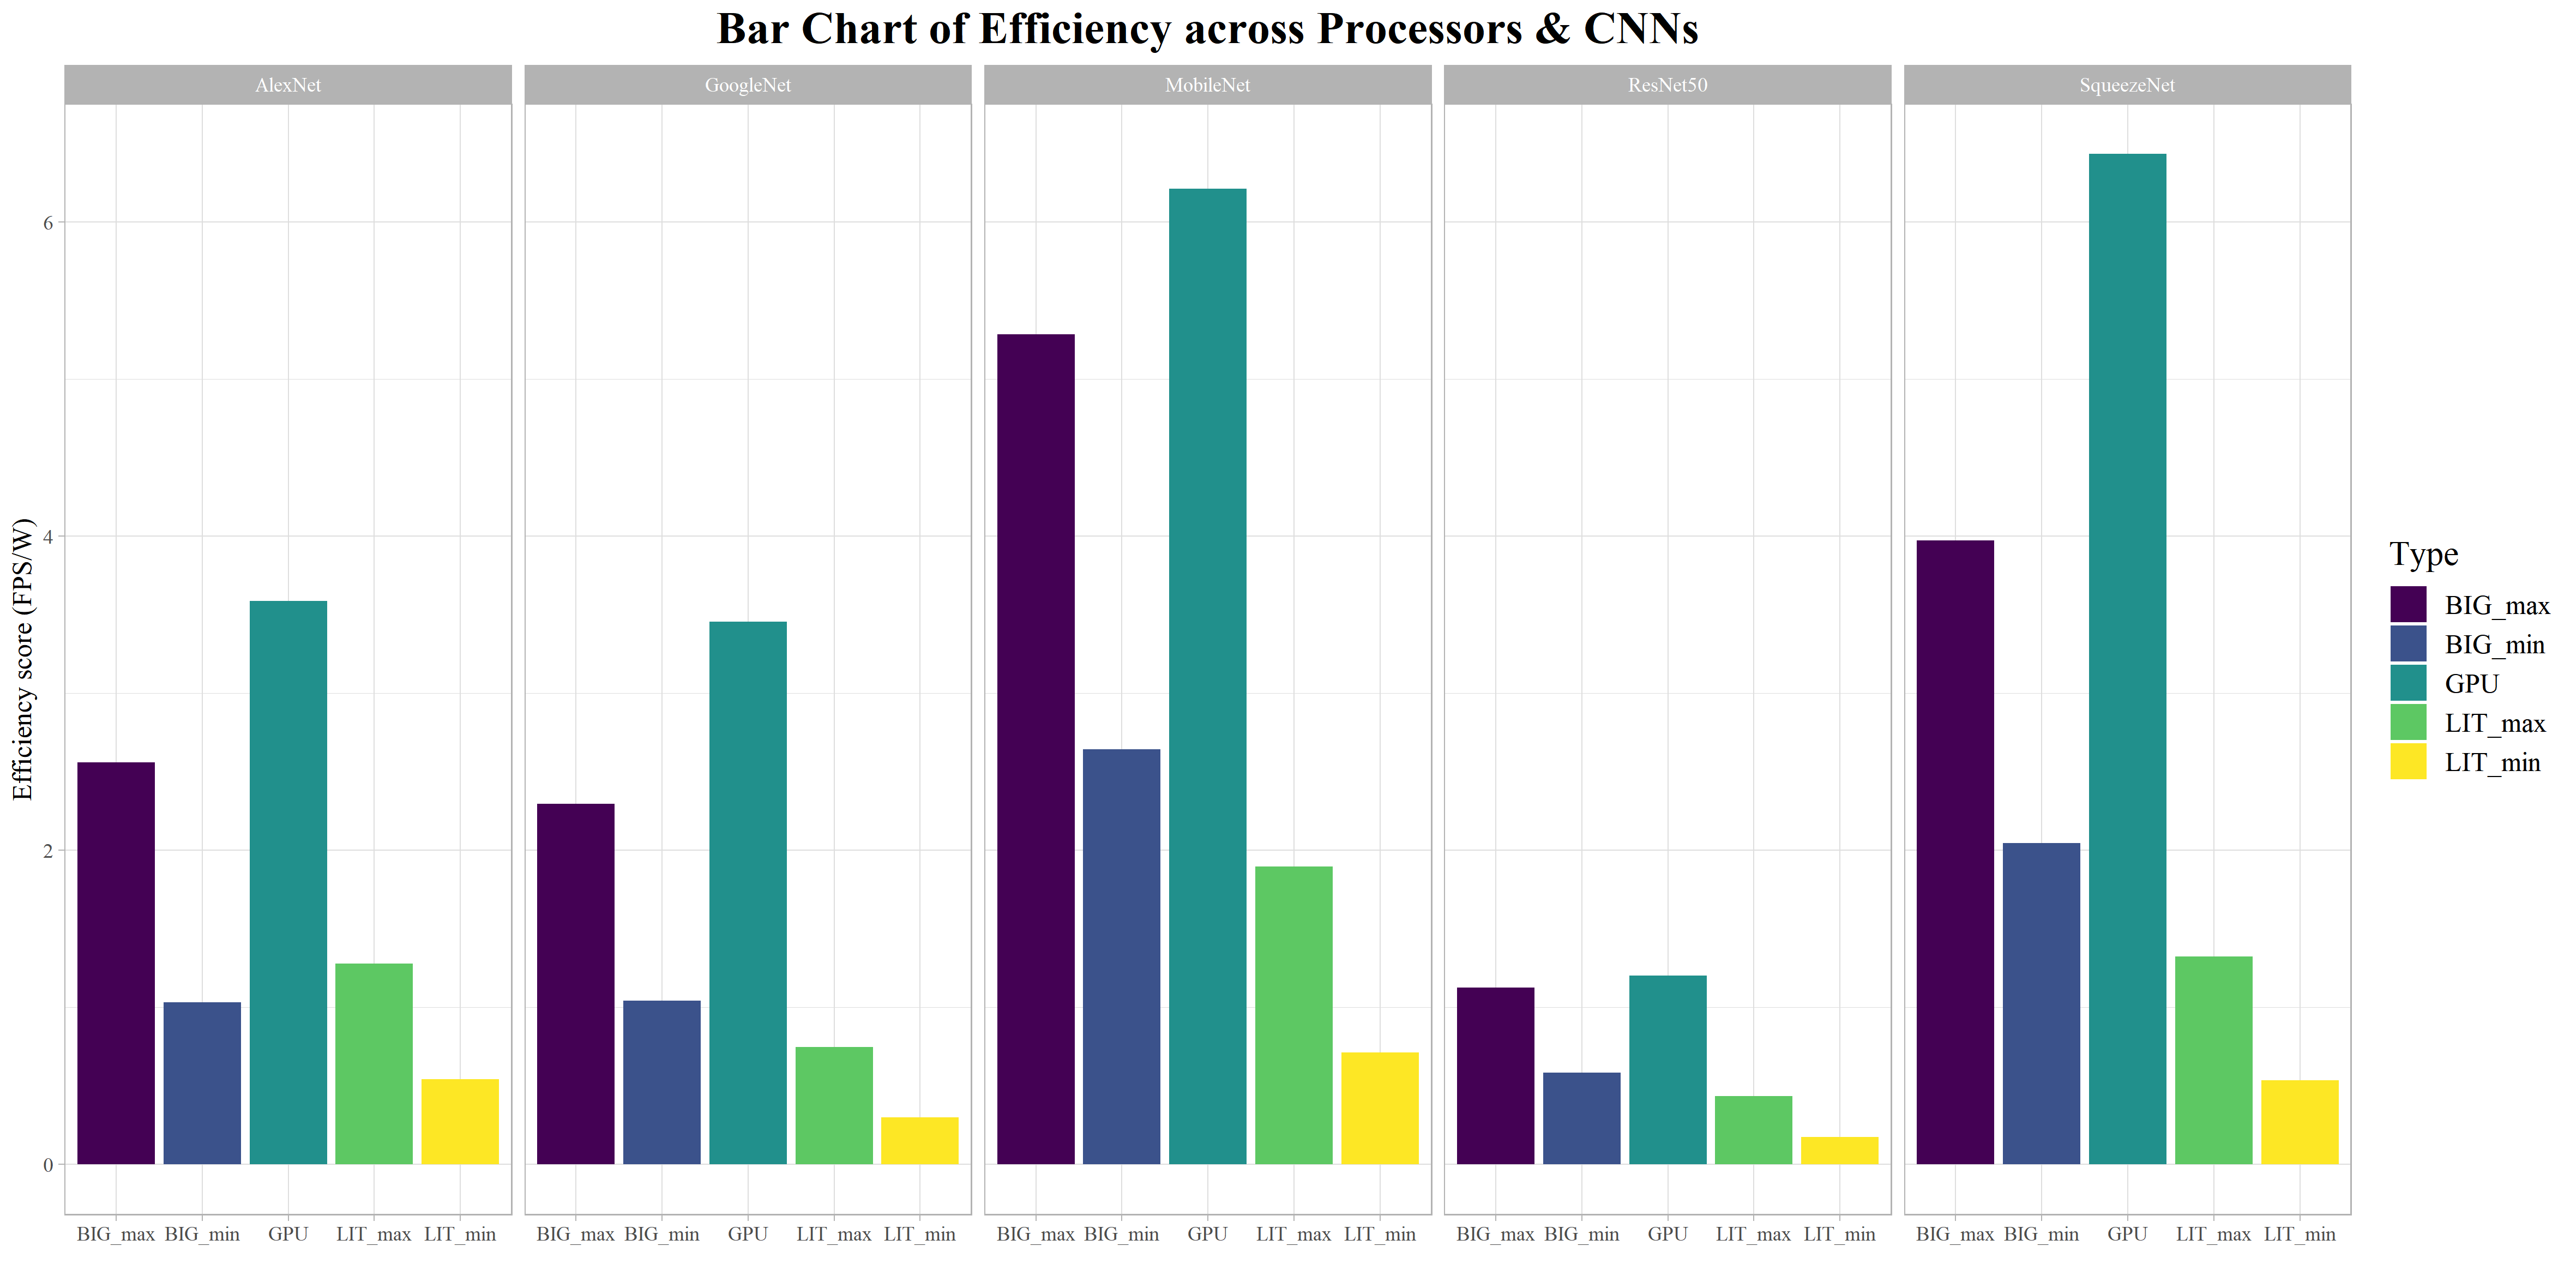
\includegraphics[width=1\linewidth]{Bar/efficiency.png}
    \caption{Efficiency Scores of the 5 CNNs}
    \label{fig:my_label}
\end{figure}

When we analyzed the data from our second set of experiments, which focused on the impact of the order of the processors on power consumption and performance, we obtained several notable observations. One of the main findings was the occurrence of a phenomenon referred to as "Process Bottleneck" or "Congestion", where a less powerful process becomes a bottleneck as it is placed before a more powerful one in the pipeline. This resulted in long wait times at the more powerful core, resulting in a temporary loss of power and a decrease in performance and latency. This effect was observed when the more powerful core was before the less powerful core, with the more powerful core completing its tasks quickly and the less powerful core being left to do the remaining work, resulting in a similar power drop. Essentially, the cycle time increases as the workloads resulted from the partitioning are unequally allocated between stages, resulting in process bottleneck.

Our data also showed that the difference in the number of operations in certain parts of a CNN has an impact on the performance and process time of the pipeline. We observed that when all parts were allocated to one of the processors, the total inference time remained constant regardless of the order of the remaining processors. However, when the orders of the working processors in the two-processor and three-processor pipelines were changed, various impacts on inference time were observed. For example, when the Little core was placed before either the other two processors, an apparent change in total inference time was observed. Additionally, when the GPU and Big CPU were swapped around, the difference in the change in performance was generally minimal, although there were cases of notable differences.

\begin{figure}[ht]
    \centering
    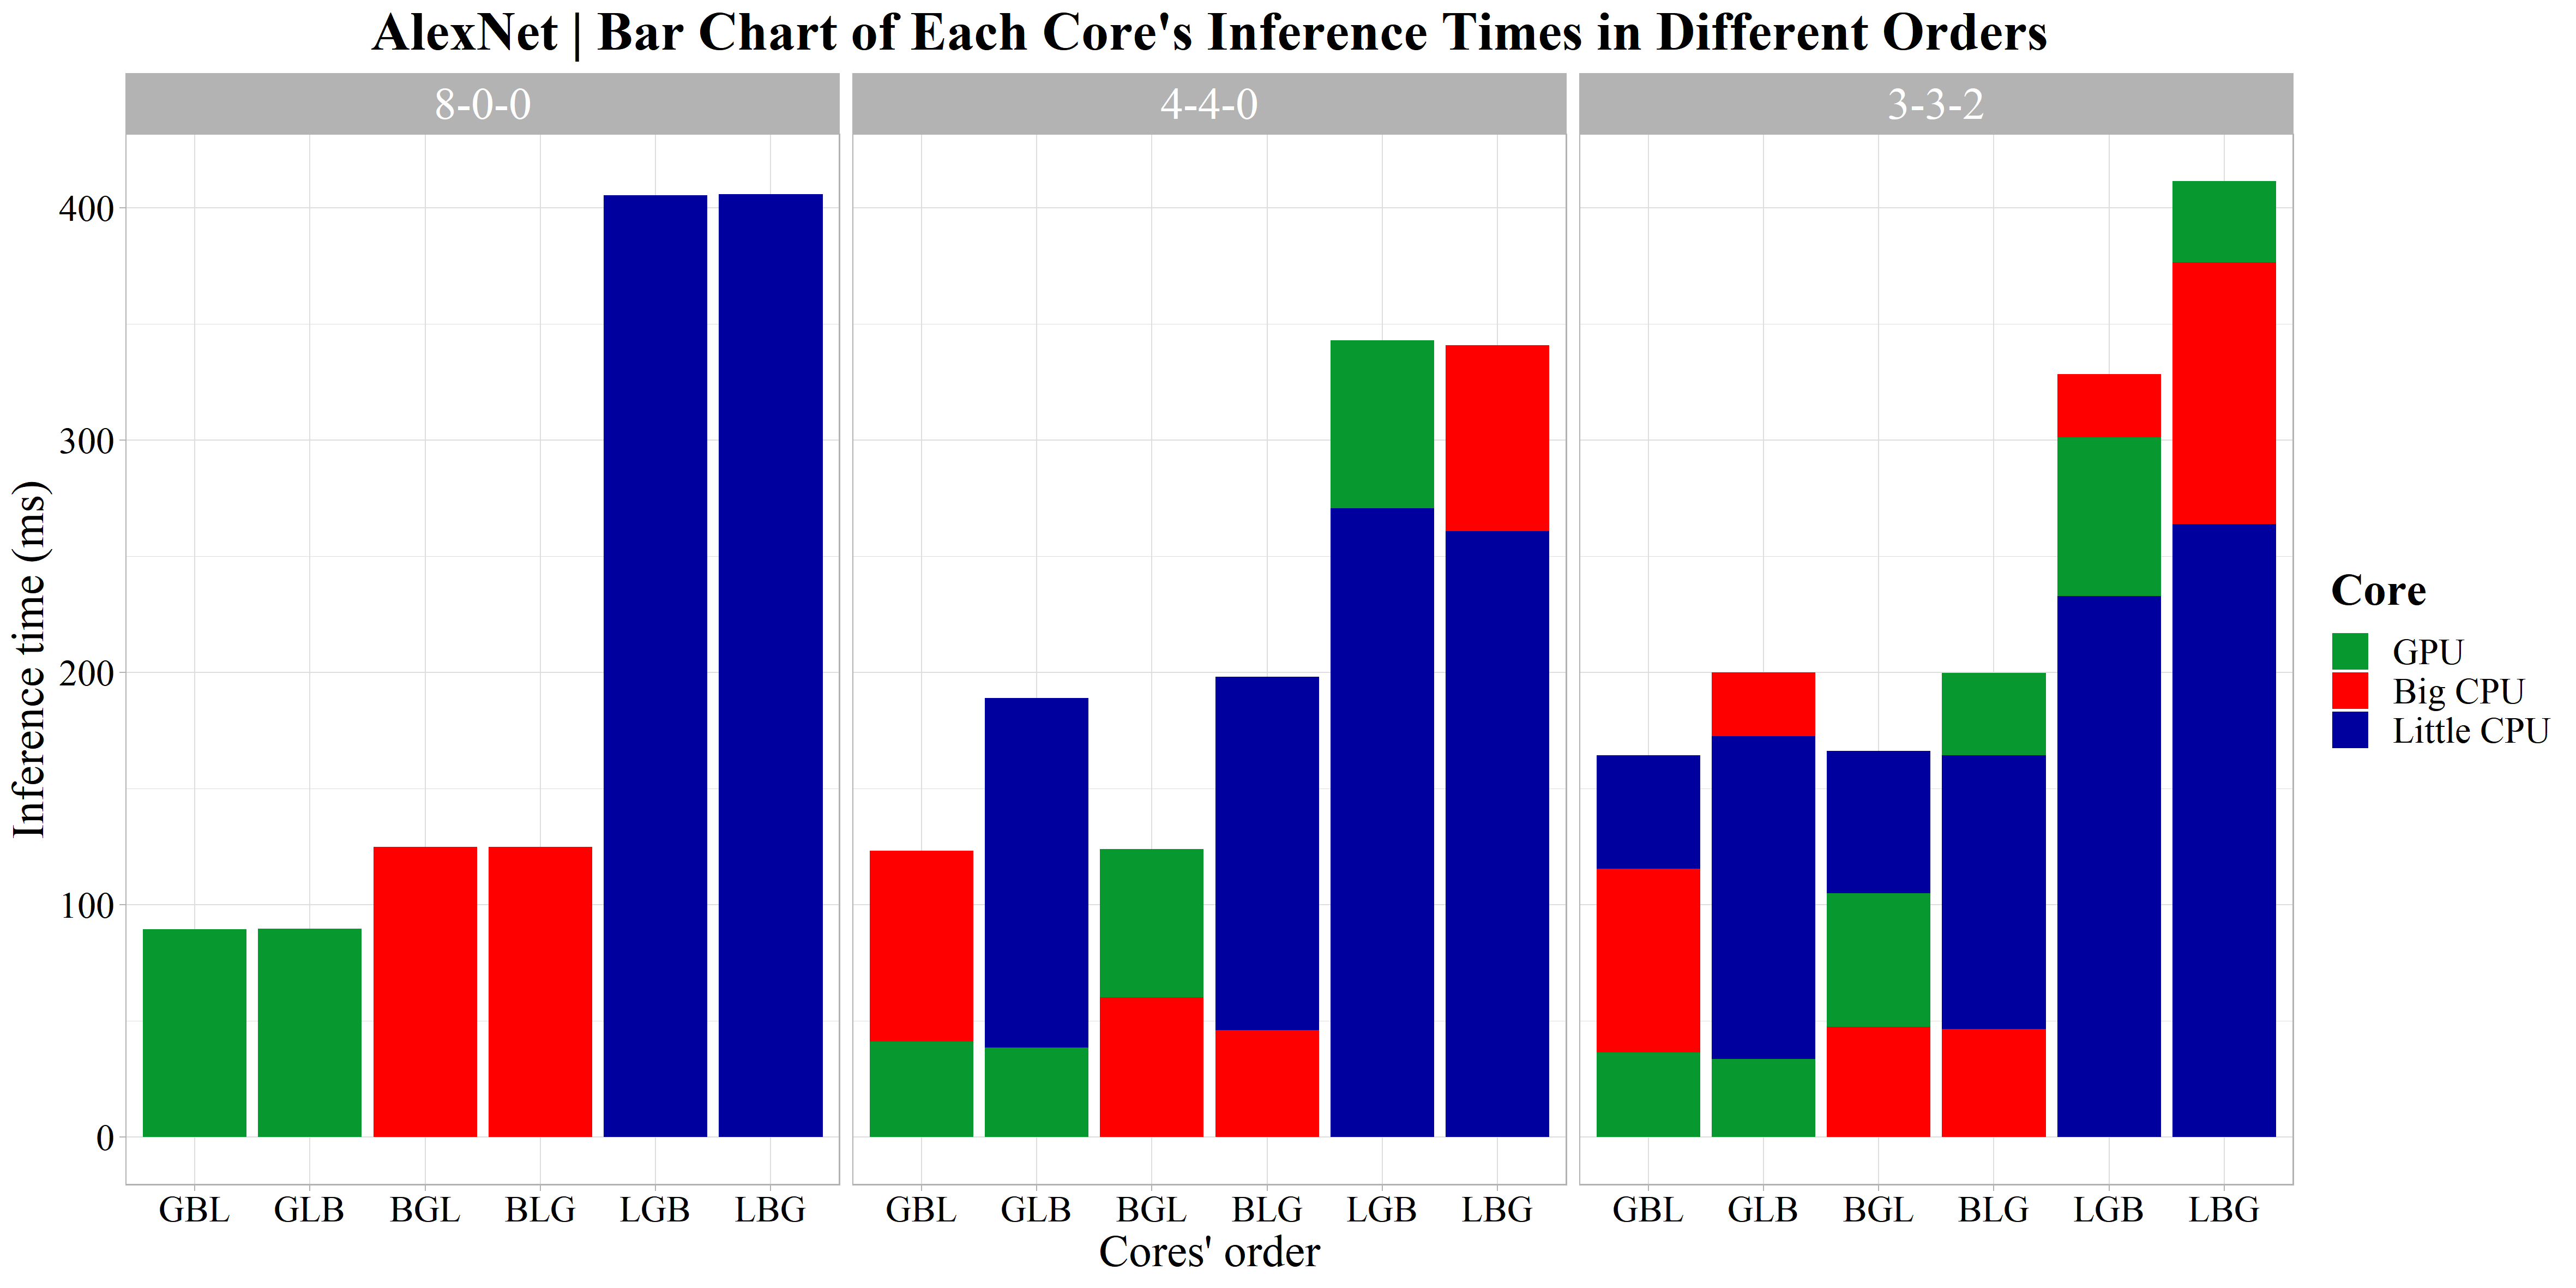
\includegraphics[width=1\linewidth]{Orders/AlexNet3.png}
    \caption{Inference time of different orders of AlexNet}
    \label{fig:f6}
\end{figure}


\begin{figure}[ht]
    \centering
    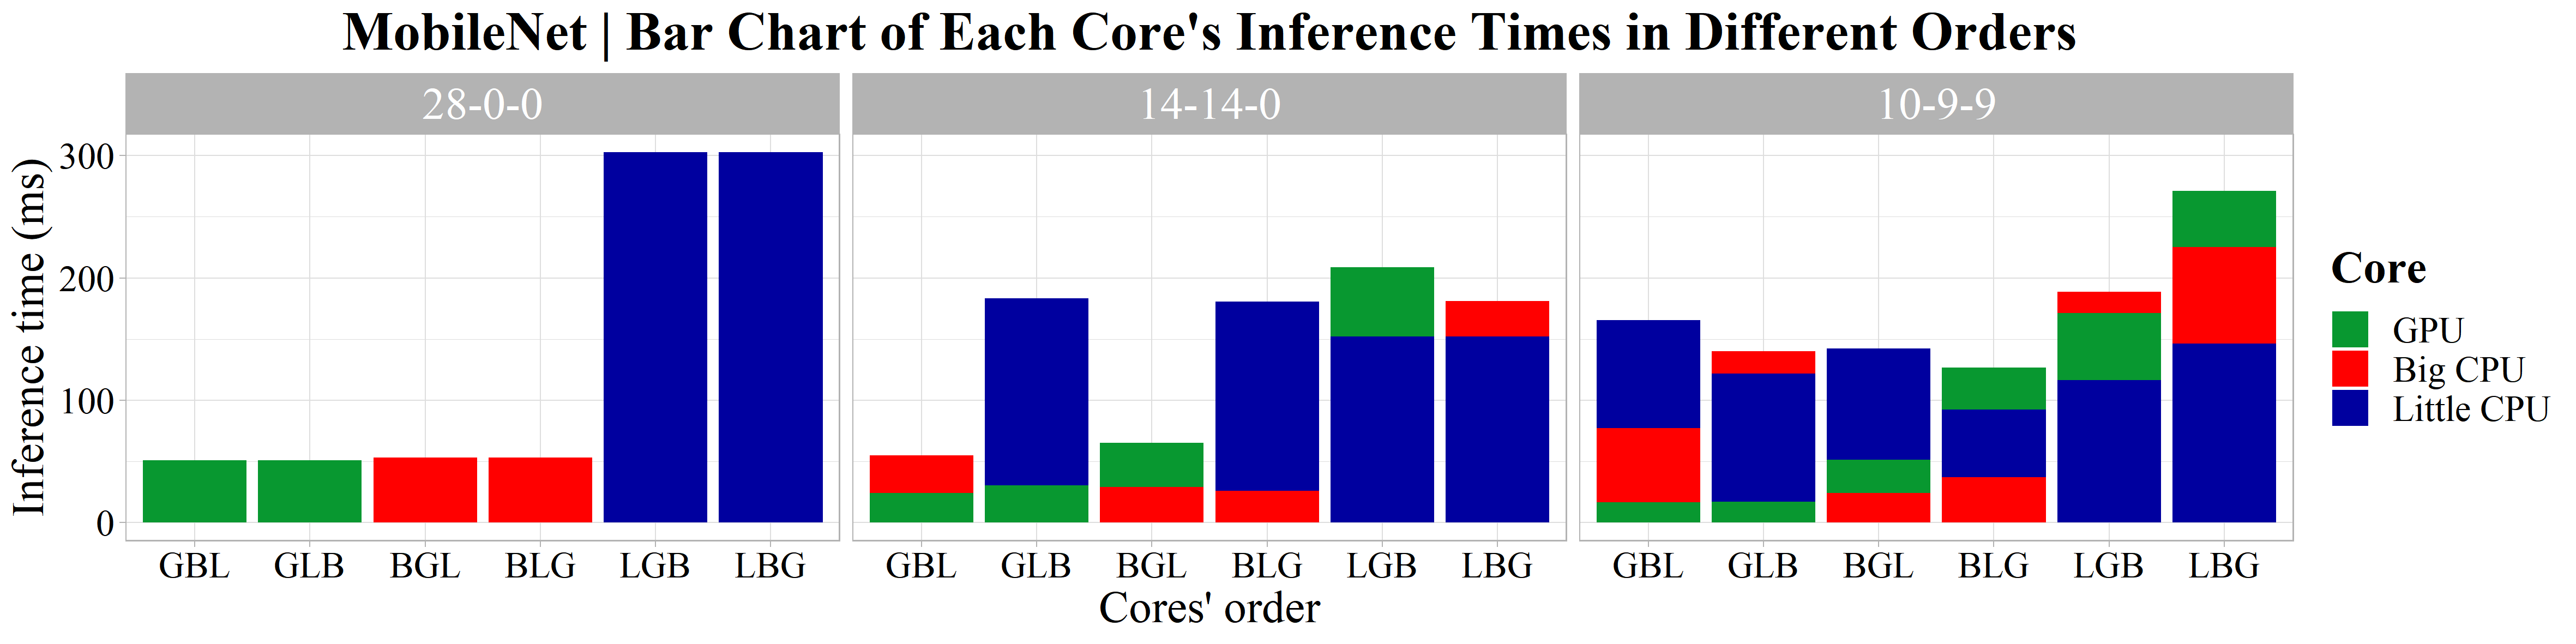
\includegraphics[width=1\linewidth]{Orders/MobileNet3.png}
    \caption{Inference time of different orders of MobileNet}
    \label{fig:f7}
\end{figure}

In terms of performance, when the total workload was divided evenly between the Big CPU and GPU, the Big CPU was able to reach the same performance as the GPU. However, this positive performance dissipated in the case of MobileNet, regardless of having the same number of parts. This showed that the difference in the number of operations in certain parts of a CNN has a significant impact on the performance and process time of the pipeline, and led us to further investigate into the partitioning of the CNNs’ parts to evaluate the number of operations in specific areas of the CNN (for instance, Figure 8 of GoogleNet).

\begin{figure}[ht]
    \centering
    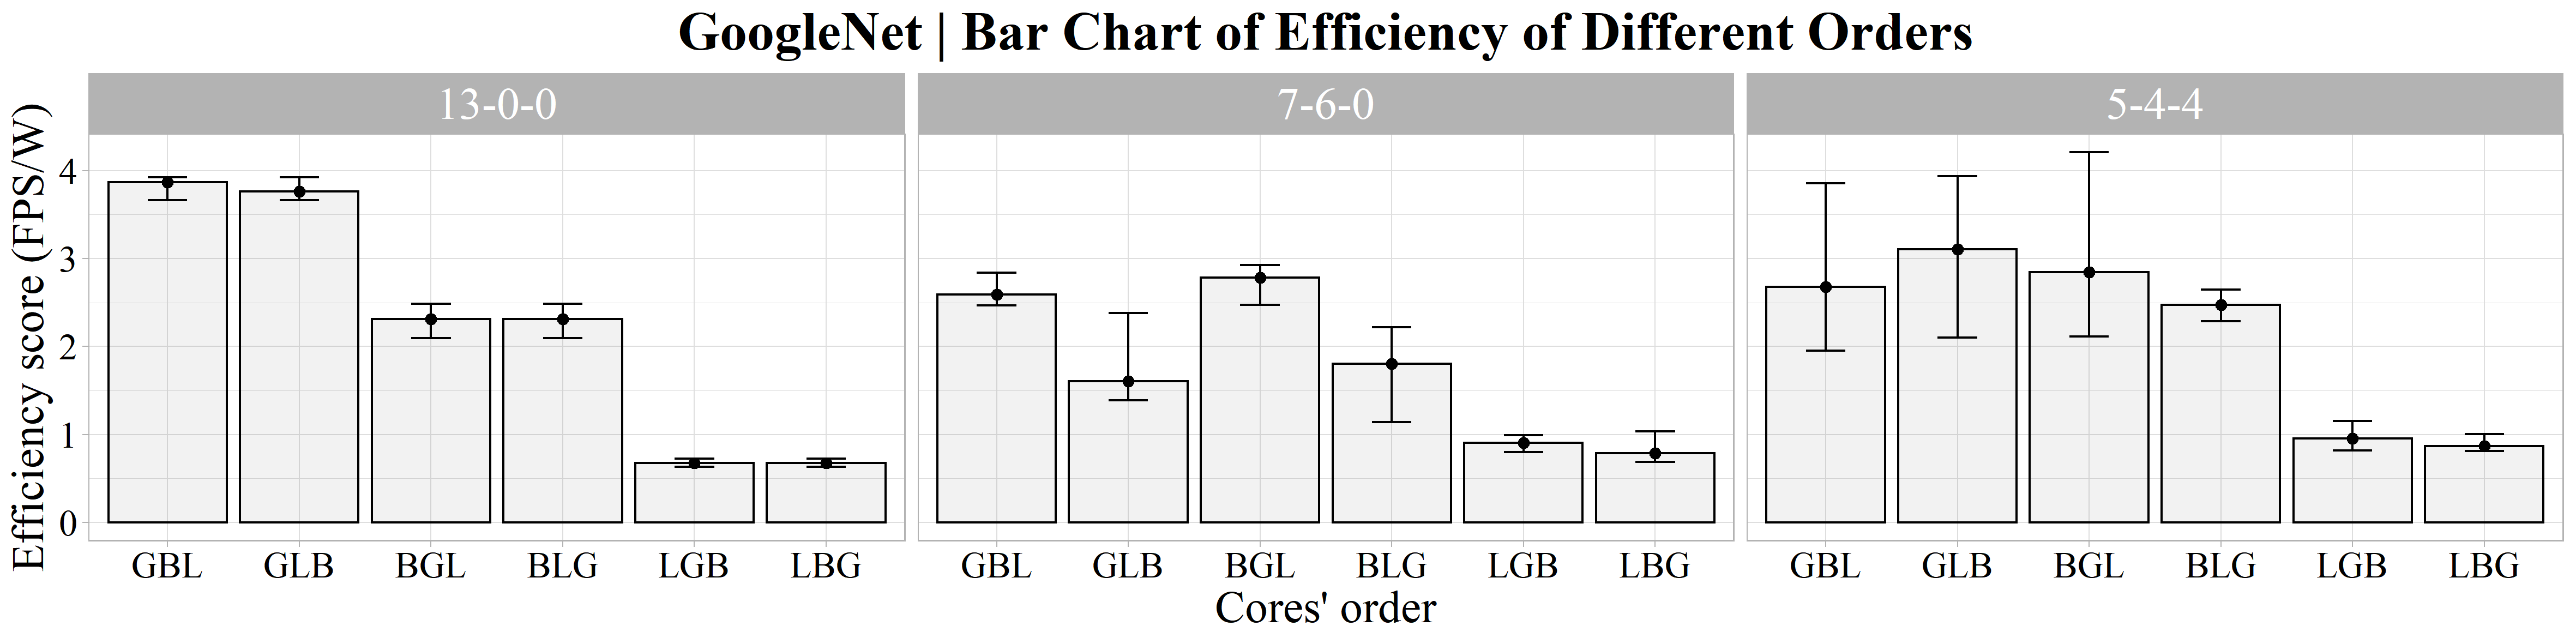
\includegraphics[width=1\linewidth]{Orders/GoogleNet3_eff.png}
    \caption{Efficiency Scores of different orders of GoogleNet}
    \label{fig:f8}
\end{figure}



\section{Conclusion and Discussion}
The power-performance characterization of CNNs on the Khadas VIM 3 board revealed a strong relationship between power consumption and performance level. As the frequency of the Big CPU cluster was increased, the frames per second (FPS) and the average frame latency improved, but the power consumption also increased. This relationship was observed for both AlexNet and GoogleNet, with GoogleNet generally having higher power consumption and lower latency than AlexNet.

The data also showed that the maximum frequency level had a greater impact on power consumption than the median or minimum values. This suggests that the board's governor and power management knobs are effective in controlling the power consumption at high-frequency levels, but may not have as much impact at lower levels.

So a other thing that looked interesting is that certain frequencies seem to have a bit of a break in use of  more power. We can see this in the big core at the kink in the line but also googlenet has one and seem to be at the same frequency. this would mean that certain features work better on frequencies that this processor likes. this could be a few features on the A73 that the A53 doesn't have. Like the more piping and the better branch prediction. Just seem to get design with these frequencies at mind. Or that the algorithms did use them more but evidence of that was not really what we found in looking at the CNN papers.

It is also important to note that the power consumption and performance levels varied between the different CNNs. For example, MobileNet v2 had lower power consumption and higher FPS than AlexNet and GoogleNet, indicating that it may be a more power-efficient option for the specific proccessors on the Khavas Vim 3.

Overall, the results of this power-performance characterization demonstrate the importance of considering power consumption when selecting CNNs for deployment on the Khadas VIM 3 board. The use of different CNNs with different architectures and configurations can have a significant impact on the power consumption and performance levels of the board.

The data collected in this report can be used as a reference for selecting the most power-efficient CNNs for different use cases on the Khadas VIM 3 board. Also some of the efficenty of diffrent CNN are diffrent meaning some can better use  a diffrent core for diffrent parts if they want a bit more performance out of as little W as possible. It's also important to consider the trade-off between power consumption and performance when adjusting the frequency of the CPU clusters.

In the future, it would be beneficial to conduct similar characterizations on other platforms and devices to understand the general trends in power consumption and performance for different CNNs.

On the charts and graphs, it is possible to see the performance of each CNN as the frequency changes, and how the power consumption changes accordingly. Each graph shows the correlation between power consumption and performance, highlighting the trade-off between the two. The data allows to identify the most power-efficient CNNs for specific use cases, and the best frequency settings to achieve the desired balance between power consumption and performance.

\section{References}
Aghapour, E., \& Torab, A. (2022). Pipe-All: High-Throughput, Low-Latency Pipelined Inference on Heterogeneous Multi-Process

\end{document}
